% Chapter submission guide:
% https://docs.google.com/document/d/1Yui8fuxUEiMsIX2G-oKfUs3vObPXb2VzKi2CKvzAg3o/edit?tab=t.0

% Suggested length: 2-10 pages (500 words per page)
% = 1000 - 5000 words

% Chapter 1 example in PP book (Charlotte et al): 
% https://pairprogramming.ed.ac.uk/chapter-students-about-pair-programming/

\section{Introduction}
% What is this chapter? (very brief)

This chapter is designed to serve as a brief tour of connections between sound, music, programming and pedagogy. In particular, it is aimed at educators who want to explore sound and music in their programming pedagogy. The chapter presents motivations for connecting these domains, introduces prior work in this area, and presents a range of \href{}{accompanying resources} that can be taken up or adapted to bring sound and music into coding education. 

Making code that makes sound and music can be fun, even with only a very basic understanding of programming concepts, and regardless of any prior music education. There are many ways in which sound and music may connect with programming. For example:

\begin{itemize}
    \item composing with code: using code to write pieces of music,
    \item performing with code: writing code in a performance to make music,
    \item creating instruments: building software tools for personal music making or for others to use,
    \item understanding sound: coding to analyse and explore representations of sound and/or music,
    \item data sonification: representing existing data as sound or music, either in real-time or with historical data,
    \item coding responsive sound and music to games or other interactive programs.
\end{itemize}

Section \ref{sec:why} explores motivations for connecting music with programming. A brief overview of the rich existing work in this domain is presented in Section \ref{sec:literature}. The set of practical accompanying resources that can serve as starting points into different kinds of music/coding projects are then introduced in Section \ref{sec:resources}. 

% Section \ref{sec:advice} presents a single piece of advice from each author from our range of different perspectives on the interconnections of sound, music, programming and pedagogy.

% Finally, Section \ref{sec:resourcetable} provides a list of possible starting points for working with sound and code.

% Resources - useful to help students with something that is already concrete and understandable.

% Music and computers have a long history together. Musicians have been making sounds by programming computers since the early 1950s (CITATIONS), both to synthesise digital sounds and to explore new approaches to composition. 





\section{Why combine programming with sound and music?} \label{sec:why}

Music and programming have a rich intertwined history. Simple but effective connections can be found between programming concepts --- such as iteration, abstraction, conditionals, loops --- and musical concepts such as rhythm, timing, harmony, pattern and so on. Writing a program that generates sound provides an immediate, engaging way to manifest abstract processes. In a pedagogical sense, the sound output is a form of feedback. Programs don't have to be complicated or sophisticated in terms of the coding to be musically satisfying. Students can create sound and music that they can share with friends and relatives, who may not know the first thing about programming but can nonetheless engage with the creative outcomes. 

% Something about UK HE policy on integrating art and science?

Programming concepts can be playfully explored in musical contexts. For example, an integer array can be rendered as a piano melody, a drum rhythm, or directly as a sound file (see Figure \ref{fig:arrays-as-music}). This gives an immediate meaning to the output data, motivating students to care about the specific values in the array, the length of the array, the range of data in the array, different ways of reading and writing values to and from the array and so on. Operations on that array take on musical meanings: ordering an array provides a scale; reversing an array reverses musical material. Meaningful data that students care about can motivate students to find things out for themselves, and provides a scope for the kind of creative explorations that are often lacking on introductory programming courses \cite{sharmin_creativity_2021}.

Sound and music can also be used to present and experience data in different ways. Data sonification has a long history \cite{worrall_2019}, from giving a constant awareness of something otherwise invisible with geiger counters or medical monitoring devices, to hearing emergent behaviours in dynamical systems, providing auditory graphs for the visually impaired \cite{walker_mauney_2010}, or creative projects that use the data for musical ends \cite{bulley_jones_2011, barrett_mair_2014}.

% QUESTION TO ALL:
% Can you think of any ways to neatly visualise this kind of thing?
% I've added something here, but let me know if you have something neater!

\begin{figure}
    \centering
    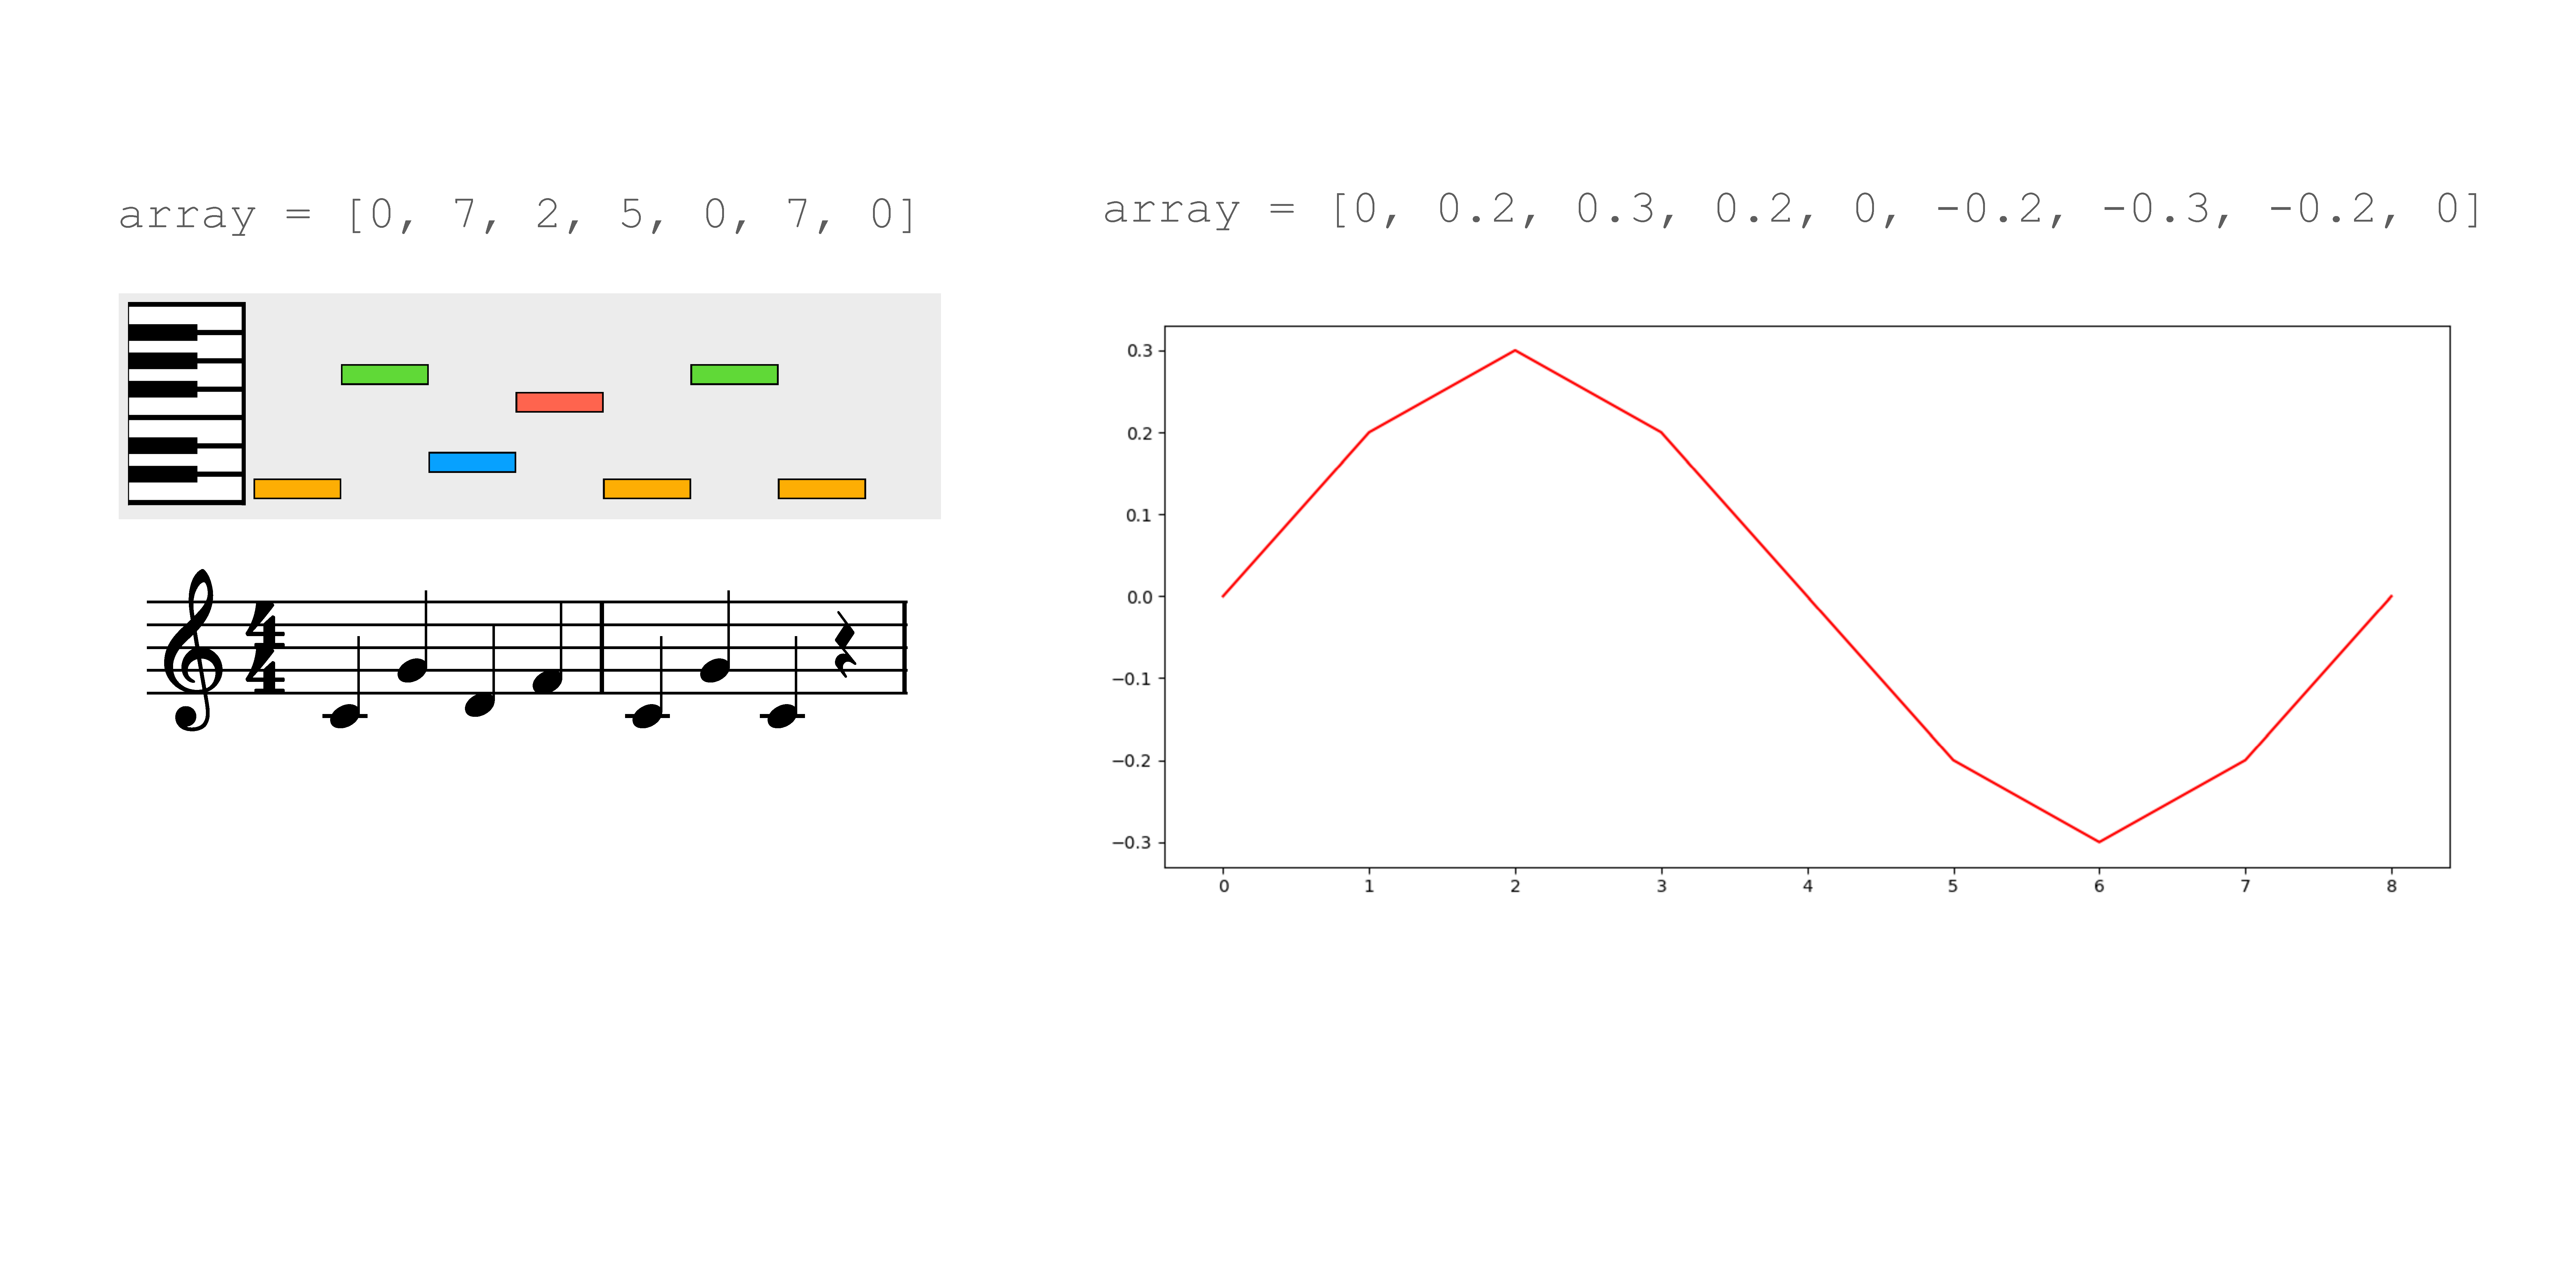
\includegraphics[width=1\linewidth]{images/fig1_arrays_as_sound_and_music.pdf}
    \caption{Two examples of arrays becoming sound and music. On the left, the array is translated into note values. On the right, the array is translated directly to an audio file.}
    \label{fig:arrays-as-music}
\end{figure}

There are obvious parallels here with coding and visual art. Environments such as Processing \cite{reas2006processing} connect programming with image and animation to motivate learning and exploration (CITE). As explored in the following section, there is a similarly rich history of music making in programming pedagogy. To mix music, art, computers and coding therefore continues a long and fruitful tradition \cite{reichardt1971, Dreher2014, wang17}, and can serve as a reminder to both students and educators that coding is fundamentally about making things and is a creative act.



% Music to teach/engage with simulation (Mike, Charlotte). Fourier transform as a nice transferable example...


\section{Overview of what exists already} \label{sec:literature}

Music and programming have been connected in a wide variety of ways, sometimes through the addition of libraries for integrating musical inputs and outputs with existing languages, and sometimes through the development of specifically designed languages or environments. As this is a very short chapter, it only scratches the surface of many of the interesting work done in this domain, and the focus is on music/code projects with explicitpedagogical elements aims.

Most mainstream programming languages are able to work with sound and music as outputs. This could be achieved by writing data to a file, e.g. an audio file [INSERT NOD TO RESOURCES] or a MIDI file (a common musical data format that can be used to synthesise sound). The program could also transmit real-time messages to an audio engine that runs separately, e.g. a standalone synthesiser or sampler \footnote{Lots of open source synthesisers are available such as \href{https://surge-synthesizer.github.io/}{Surge XT} or \href{https://asb2m10.github.io/dexed/}{Dexed}}, a digital audio workstation, or frameworks such as \href{https://github.com/musikinformatik/SuperDirt}{SuperDirt}. Most mainstream programming languages will have libraries available for these purposes, making it relatively easy to adapt any simple programming exercise into a sonic/musical exercise. % e.g. adding an element to array could be adding a note to a melody or conditional statements might be musical decisions.


The Scratch programming language\footnote{\url{https://scratch.mit.edu/educators/}} is a well established starting point for young people to engage with coding. While sound and music are not usually the primary focus for students, there is still considerable scope for creativity and experimentation. Brown and Ruthman present a useful range of project types in their \emph{Scratch Music Projects} book \cite{brown20}, from simple theremin-like interactive instruments, through playing simple riffs, up to thinking about loops, musical structures, generative music, and live coding performance. As Scratch is used more generally for creating games, stories or animations, students can be motivated to explore sound and music as one component in wider creative projects.

Sonic Pi\footnote{\url{https://sonic-pi.net}} is a popular example of a language specifically designed for music. It is a simple but flexible environment that aims to support school-age students to learn to code by making music \cite{aaron_sonic_2016}. As with Scratch, the focus on play and having fun with Sonic Pi can foster a more positive attitude towards programming \cite{petri_sonicpi_2022}, and can provide a starting point for moving from simple programming concepts to more involved topics such as concurrency \cite{traversaro_hearplay_2024}. Sound-making programs can start off very simple with basic commands such as "play 60", but can be built into entire pieces or performances \footnote{e.g. see work by DJ\_Dave in Sonic Pi \url{https://www.youtube.com/watch?v=w2s1DK1w3WI}}. 

Sonic Pi is rooted in practices of live coding for music, a substantial community that serves as an access point to programming for many musicians, as well as an access point for music for some programmers. The movement has engaged closely with programming pedagogy from different perspectives; Blackwell et al \cite{blackwell_livecoding_2022} provide a useful overview. The proceedings of the International Conference on Live Coding\footnote{\url{https://iclc.toplap.org/}} also present a broader repository of topics, many of which cover music in programming education (GIVE EXAMPLES). Live musical coding is also notable as a community that has attempted to push back against coding as a male-dominated space \cite{blackwell_livecoding_2022}, with all-women and non-binary workshops being a regular occurrence. Armitage \cite{armitage_spaces_2018} points to the domain as being a ``a space in which to fail constructively''.

The EarSketch\footnote{\url{https://earsketch.gatech.edu/}} \cite{engelman_earsketch_2017} and TunePad\footnote{\url{https://tunepad.com/}} projects are similar to Sonic Pi in their pedagogical aims, in that they seek to broaden participation in computing by demystifying coding and relating it to a domain of interest to students. The projects embed coding elements alongside more conventional music-making tools such as tracks, instruments, timeline, mixer, etc.  This provides a familiar workspace for those with musical backgrounds and means that the code doesn't need to cover all aspects of the music making, but can be written in snippets with very particular goals, such as making a drum loop, or a bass riff. Both projects run in the browser and use Python (although EarSketch has a JavaScript option). They are designed specifically with sharing in mind: both code sharing and collaborative editing, further motivating students to engage with the coding \cite{freeman_earsketch_2019}. Petrie \citep{petrie_ct_2024} studied the potential for both projects to support computational thinking in 11-12 year old students who had no prior school experience of either programming or music making. Petrie notes that students benefit from the fact that the kinds of musical tasks supported by these projects are naturally incremental and iterative.

% STRUDEL / TIDALCYCLES? 


A key concern across all the above projects is that there should be room for musical variety and expression; although they may present simple entry points to engaging with programming, it is possible to create rich and interesting creative work that students will be proud of.



\section{Overview of our online resources [rename this]} \label{sec:resources}
%What are they, who are they for, what kinds of programming concepts do they relate to?

% Our working list of projects is here:
% https://docs.google.com/document/d/1FsmVMrJlf2lRL4Jb25oat9y6M3Uvrkz7JEuytC6oyb8/edit?usp=sharing

% Include a list of resources for how you might adapt some of these examples to other libraries?
% E.g. midi library things, audio read/write libraries, etc.
% Other guides to setting up where these exist already.

Perhaps a quick note towards the many many things that are important, but perhaps out of scope here.

Five example resources accompany this chapter that reflect some of the different approaches to combining aspects of sound, music and programming in the different authors' pedagogical work. Each example resource comes with a readme that gives a sense of how the resource might be used, who might find it valuable, what prior knowledge the students may need, and what technologies will be needed.

\subsection{Python piano piece}
This resource is aimed at students who have started on Python quite recently. It attempts to make musical output as simple and accessible as possible. Students are shown how to generate piano pieces as MIDI data which can be played back directly within a Python notebook. Students can develop their understanding of fundamental concepts programming concepts such as lists, loops and conditionals. The ability to directly hear the results is intended to motivate students to think about how they can develop the code by themselves to try to explore how they can start to tailor the musical output towards something they find sonically interesting or satisfying.

\subsection{Strudel drum patterns}
This resource is both similar and different to the piano example. Students engage with \emph{Strudel}\footnote{\url{https://strudel.cc/workshop/getting-started/\#what-is-strudel}}, a browser-based JavaScript port of the popular \emph{TidalCycles}\footnote{https://tidalcycles.org/} live coding language. The language has been particularly popular for exploring algorithmic approaches to beat making\footnote{see the international Algorave movement for example: \url{https://algorave.com/}}. The editor provides useful visual feedback to show how the code relates to the unfolding beats. It has been a popular way to engage with code for the first time for many \ref{CITATION}, as well as being an useful introduction to Haskell and functional programming for others \cite{CITATION}. Unlike the Python example above, it may not be so straightforward to map programming insights directly to other domains such as data science or INSERT ANOTHER DOMAIN HERE.

\subsection{[Charlotte]}
% Short overview goes here


\subsection{[Matthew]}
This section focusses on educators directly and the ground work needed to make the most portable and technologically accessible lessons. No prior knowledge is assumed and as the resource is intended to guide the reader through the process of WAVE file creation. The ultimate goal being a simple library ripe for customisation and intimately understood for easy dissemination to students.

All data can be a sound and the WAVE file is the simplest means of data sonification and music creation. Most modern operating systems (and many older ones) will support WAVE file playback through a media player, browser or command line tool. The resource emphasises the use of standard libraries to improve portability and providing a means of quickly beginning music-based programming lessons without burdening students with language-specific ancillary concepts that can potentially be a demotivating obstacle to new programmers.

The intention is not to be prescriptive, but rather show how malleable the WAVE format can be for teaching music and programming.

% want to talk about twos compliment? great, talk about signed integers and bit-depth. Want to talk about additivie synthesis? lovley, stack sine waves and put them in a .wav. Want to talk about Redbook audio, CD formats and PCM?  I wanetd emphasise here just how customusable such a simple basic concept (in computer science terms) and is stil very relevant. Basically almost like the WAVE file isn't the important bit, but the philosophy behind the decisions for teaching it.

The central lesson is explained in an IPython (Jupyter) notebook, but there is also companion code in C, C++, Java and Rust to reinforce the basic elements need to solve the problem.

% list of places to go, adding functionality to the library or expanding on the base WAVE format to include other chunks such as cue and playlist chunks which could be used in conjunction with Adobe Audition, Avid Pro Tools, Steinberg Cubase/Nuendo, REAPER, Presonus Studio One FL Studio, samplers Akai MPC, Kontakt or with FMOD or WWise for creating loop points. https://www.mmsp.ece.mcgill.ca/Documents/AudioFormats/WAVE/Docs/riffmci.pdf

\subsection{[Mike]}
% Short overview goes here

\subsection{[Yash]}
This demo serves as a template or a starting point to create web-based responsive musical instruments and/or controllers. The template combines RNBO (by Cycling '74) (link?), using JavaScript and smartphone sensors, to build a responsive synthesiser hosted on the web that, when accessed from a smartphone, utilises the motion sensors to control specific parameters of the synthesiser. It features a simple RNBO Additive synth patch with some simple effects like distortion and EQ. The audio engine is exported from RNBO and embedded into a lightweight HTML/JavaScript site inspired by Cycling ’74’s example code, with unnecessary UI stripped away for clarity. A p5.js-based sequencer for playing notes and visual feedback. Motion data from a smartphone’s orientation sensors is mapped in real time to RNBO parameters, enabling gestural control over sound, allowing gestures like tilting or twisting a phone to shape the sound. Designed as both a learning resource and a creative springboard, the project can be adapted for musical instruments, live installations, audience-participation performances, or experimental audio-visual tools.


\section{Mini summary}
This chapter has touched briefly on some of the many connections between sound, music and programming that exist, and how these can be and have been productively brought to bear on programming pedagogy. 


% too much?
We close with Rebecca Fiebrink's advice to musical coders \cite[p 145]{brown20}, that captures some of the excitement of bringing these two domains together:
\begin{quote}
    Have you figured out how to recreate your favorite pop song with code? Great! Now try composing a new song that's all your own. Or see if you can create new types of music that are easier to make with code than without it --- or even types of music that are impossible to create without a computer! What do you come up with? Can you make new sounds that nobody in the world has ever heard before? Can you make musical “instruments” that you can interact with to perform music that you could never make with a piano or a violin? What else could you create, that nobody before you has ever made?
\end{quote}

\section{Resource List for educators}

% TABLE
% ADD:  
%% library for C++
%% 


  

% \begin{table}
%     \scriptsize
%     \centering
%     \begin{adjustwidth}{-2cm}{-2cm}
%     \begin{tabular}{m{6em}m{7em}m{5em}>{\centering}m{5em}m{5em}m{6em}m{7em}}
%     % {ccclcll}
%          \textbf{Name} & \textbf{Type}& \textbf{Context}& \textbf{Open Source}& \textbf{Notes}& \textbf{Audience}& \textbf{URL} \\
%          &  &  &   && &\\
%          EarSketch&  Browser-based&  Beginner music making&   &Python or JavaScript& &earsketch.gatech.edu\\
%  gm (R)& R music library& Data science& & R& &flujoo.github.io/gm\\
%          JythonMusic&  Standalone application&  Beginner music making&   &Python& &jythonmusic.me\\
%          Mido&  Python MIDI library&  Beginner music making&   \checkmark&Python& &mido.readthedocs.io\\
%  Max& Standalone application, Visual coding& Music making& X& & musicians&\\
%  PureData& Standalone application, Visual coding& &  \checkmark&& &puredata.info\\
%          Scratch&  Browser-based visual coding&  Beginner music / game / animation&   \checkmark&Visual coding&  young learners&scratch.mit.edu\\
%          Sonic Pi&  Standalone application&  &   \checkmark&Ruby& young learners&sonic-pi.net\\
%          Strudel&  Browser-based port of TidalCycles&  &   \checkmark&& &strudel.cc\\
%  SuperCollider& & & \checkmark& & &\\
%          Tau5&  Browser-based or standalone application&  &  && &tau5.live\\
%  TidalCycles& live coding environment& &  \checkmark&Requires SuperCollider / SuperDirt for sound output& &tidalcycles.org\\
%  TunePad& Browser-based& & & Python& &tunepad.com\\
%  Wav libraries& Libraries for various& &  && &\\ 
%     \end{tabular}
% \end{adjustwidth}    
%     \caption{An incomplete list of software and software libraries that can be helpful in exploring music, sound and coding}
%     \label{tab:placeholder}
% \end{table}


\begin{table}
    \scriptsize
    \centering
    \begin{adjustwidth}{-2cm}{-2cm}
    \begin{tabular}{>{\raggedleft}m{6em}>{\centering}m{7em}>{\raggedright}m{5em}>{\centering}m{3em}>{\raggedright}m{5em}>{\raggedright}m{6em}m{7em}}
    % {ccclcll}
         \textbf{Name} & \textbf{Type}& \textbf{Context}& \textbf{Open Source}& \textbf{Notes}& \textbf{Audience}& \textbf{URL} \\
         &  &  &   && &\\
         EarSketch&  Browser-based&  Beginner music making&   &Python or JavaScript& &earsketch.gatech.edu\\
 gm (R)& R music library& Data science& & R& &flujoo.github.io/gm\\
         JythonMusic&  Standalone app&  Beginner music making&   &Python& &jythonmusic.me\\
         Mido&  Python MIDI library&  Beginner music making&   \checkmark&Python& &mido.readthedocs.io\\
 Max& Standalone app, Visual coding& Music making& X& & musicians&\\
 PureData& Standalone app, Visual coding& &  \checkmark&& &puredata.info\\
         Scratch&  Browser-based visual coding&  Beginner music / game / animation&   \checkmark&Visual coding&  young learners&scratch.mit.edu\\
         Sonic Pi&  Standalone app&  &   \checkmark&Ruby& young learners&sonic-pi.net\\
         Strudel&  Browser-based port of TidalCycles&  &   \checkmark&& &strudel.cc\\
 SuperCollider& & & \checkmark& & &\\
         Tau5&  Browser-based or Standalone app&  &  && &tau5.live\\
 TidalCycles& live coding environment& &  \checkmark&Requires SuperCollider / SuperDirt for sound output& &tidalcycles.org\\
 TunePad& Browser-based& & & Python& &tunepad.com\\
 Wav libraries& Libraries for various& &  && &\\ 
    \end{tabular}
\end{adjustwidth}    
    \caption{An incomplete list of software and software libraries that can be helpful in exploring music, sound and coding}
    \label{tab:placeholder}
\end{table}
